\documentclass[12pt]{article}
\usepackage{amsmath}
\usepackage{parskip}
\usepackage{graphicx}
\usepackage[letterpaper, margin=1in]{geometry}
\usepackage{fancyhdr}
\fancypagestyle{prelabheader} {
    \rhead{Raeed Hassan \\ hassam41}
    \lhead{\huge{ELECENG 2CI5 Lab 5 Prelab}}
}
\graphicspath{{./images/}}

\begin{document}
\newgeometry{margin=1in, includehead, head=47pt}
\thispagestyle{prelabheader}
i. \\
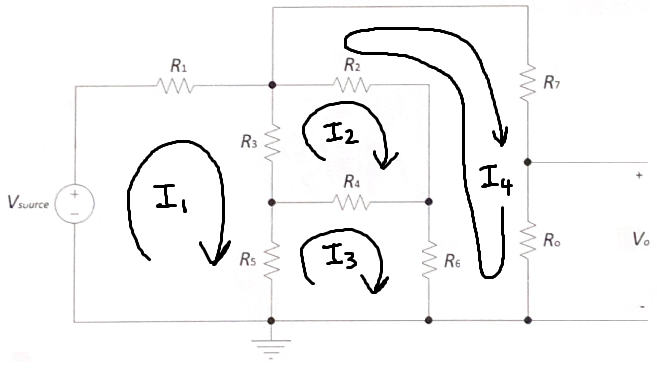
\includegraphics[width=\textwidth]{Circuit} \\

\underline{Loop 1}
\begin{equation}
    \begin{gathered}
        R_1I_1 + R_3(I_1-I_2) + R_5(I_1-I_3) = V_{source} \\
        (R_1 + R_3 + R_5)I_1 - R_3I_2 - R_5I_3 + 0I_4= V_{source}
    \end{gathered}
\end{equation}

\underline{Loop 2}
\begin{equation}
    \begin{gathered}
        R_2(I_2-I_4) + R_3(I_2-I_1) + R_4(I_2-I_3) = 0 \\
        -R_3I_1 + (R_2 + R_3 + R_4)I_2 - R_4I_3 - R_2I_4 = 0
    \end{gathered}
\end{equation}

\underline{Loop 3}
\begin{equation}
    \begin{gathered}
        R_4(I_3-I_2) + R_5(I_3-I_1) + R_6(I_3-I_4) = 0 \\
        -R_5I_1 - R_4I_2 + (R_4 + R_5 + R_6)I_3 - R_6I_4 = 0
    \end{gathered}
\end{equation}

\underline{Loop 4}
\begin{equation}
    \begin{gathered}
        R_2(I_4-I_2) + R_6(I_4-I_3) + R_7I_4 + R_oI_4 = 0 \\
        0I_1 - R_2I_2 - R_6I_3 + (R_2 + R_6 + R_7 + R_o)I_4 = 0
    \end{gathered}
\end{equation}
\restoregeometry
\clearpage
\[
\begin{matrix}
    (1) \\
    (2) \\
    (3) \\
    (4)    
\end{matrix}
\begin{bmatrix}
    (R_1 + R_3 + R_5) & -R_3 & -R_5 & 0 \\
    -R_3 & (R_2 + R_3 + R_4) & -R_4 & -R_2 \\
    -R_5 & -R_4 & (R_4 + R_5 + R_6) & -R_6 \\
    0 & -R_2 & -R_6 & (R_2 + R_6 + R_7 + R_o)
\end{bmatrix}
\begin{bmatrix}
    I_1 \\
    I_2 \\
    I_3 \\
    I_4
\end{bmatrix}
=
\begin{bmatrix}
    V_{source} \\
    0 \\
    0 \\
    0
\end{bmatrix}
\]

\[
\begin{bmatrix}
    I_1 \\
    I_2 \\
    I_3 \\
    I_4
\end{bmatrix}
=
\begin{bmatrix}
    (R_1 + R_3 + R_5) & -R_3 & -R_5 & 0 \\
    -R_3 & (R_2 + R_3 + R_4) & -R_4 & -R_2 \\
    -R_5 & -R_4 & (R_4 + R_5 + R_6) & -R_6 \\
    0 & -R_2 & -R_6 & (R_2 + R_6 + R_7 + R_o)
\end{bmatrix} ^{-1}
\begin{bmatrix}
    V_{source} \\
    0 \\
    0 \\
    0
\end{bmatrix}
\]

ii. \\
\[
\begin{bmatrix}
    I_1 \\
    I_2 \\
    I_3 \\
    I_4
\end{bmatrix}
=
\begin{bmatrix}
    (R_1 + R_3 + R_5) & -R_3 & -R_5 & 0 \\
    -R_3 & (R_2 + R_3 + R_4) & -R_4 & -R_2 \\
    -R_5 & -R_4 & (R_4 + R_5 + R_6) & -R_6 \\
    0 & -R_2 & -R_6 & (R_2 + R_6 + R_7 + R_o)
\end{bmatrix} ^{-1}
\begin{bmatrix}
    V_{source} \\
    0 \\
    0 \\
    0
\end{bmatrix}
\]

\[
\begin{bmatrix}
    I_1 \\
    I_2 \\
    I_3 \\
    I_4
\end{bmatrix}
=
\]

\footnotesize
\[
\begin{bmatrix}
    (220\Omega + 1k\Omega + 1k\Omega) & -1k\Omega & -1k\Omega & 0 \\
    -1k\Omega & (1k\Omega + 1k\Omega + 10k\Omega) & -10k\Omega & -1k\Omega \\
    -1k\Omega & -10k\Omega & (10k\Omega + 1k\Omega + 10k\Omega) & -10k\Omega \\
    0 & -1k\Omega & -10k\Omega & (1k\Omega + 10k\Omega + 10k\Omega + 24.7k\Omega)
\end{bmatrix} ^{-1}
\begin{bmatrix}
    4V \\
    0 \\
    0 \\
    0
\end{bmatrix}
\]

\[
\begin{bmatrix}
    I_1 \\
    I_2 \\
    I_3 \\
    I_4
\end{bmatrix}
=
\begin{bmatrix}
    2.227 \text{mA} \\
    0.535 \text{mA} \\
    0.409 \text{mA} \\
    0.101 \text{mA}
\end{bmatrix}
\]

iii.

\begin{tabular}{|c|c|c|}
    \hline
     & $I_{calculated}$ (mA) & $I_{measured}$ (mA) \\ \hline
    $I_1$ & $2.227$ & $2.22$ \\ \hline
    $I_2$ & $0.535$ & $0.550$ \\ \hline
    $I_3$ & $0.409$ & $0.420$ \\ \hline
    $I_4$ & $0.101$ & $0.0995$ \\ \hline
\end{tabular}

iv. \\
\[
    V_o = I_4R_o = 0.101mA \times 24.7k\Omega = 2.495V
\]
The calculated value of $V_o$ is 2.495V. The measured value of $V_o$ is 2.482V. \\
\newpage
v.
\begin{align*}
    P_o & = \frac{V_o^2}{R_o} \\ 
    P_{o_{calculated}} & = \frac{V_{o_{calculated}}^2}{R_o} = \frac{2.495^2}{24.7k} = 0.252mW \\
    P_{o_{measured}} & = \frac{V_{o_{measured}}^2}{R_o} = \frac{2.482^2}{24.7k} = 0.249mW 
\end{align*}
The calculated value of $P_o$ using the calculated value of $V_o$ is 0.252mW. The calculated value of $P_o$ using the measured value of $V_o$ is 0.249mW.

vi. \\
The measured value of $V_o$ is 0.310V. The calculated value of $P_o$ is 0.0961mW.
\[
    P_{o_{measured}} = \frac{V_o^2}{R_o} = \frac{0.310^2}{1k} = 0.0961mW
\]

vii. \\

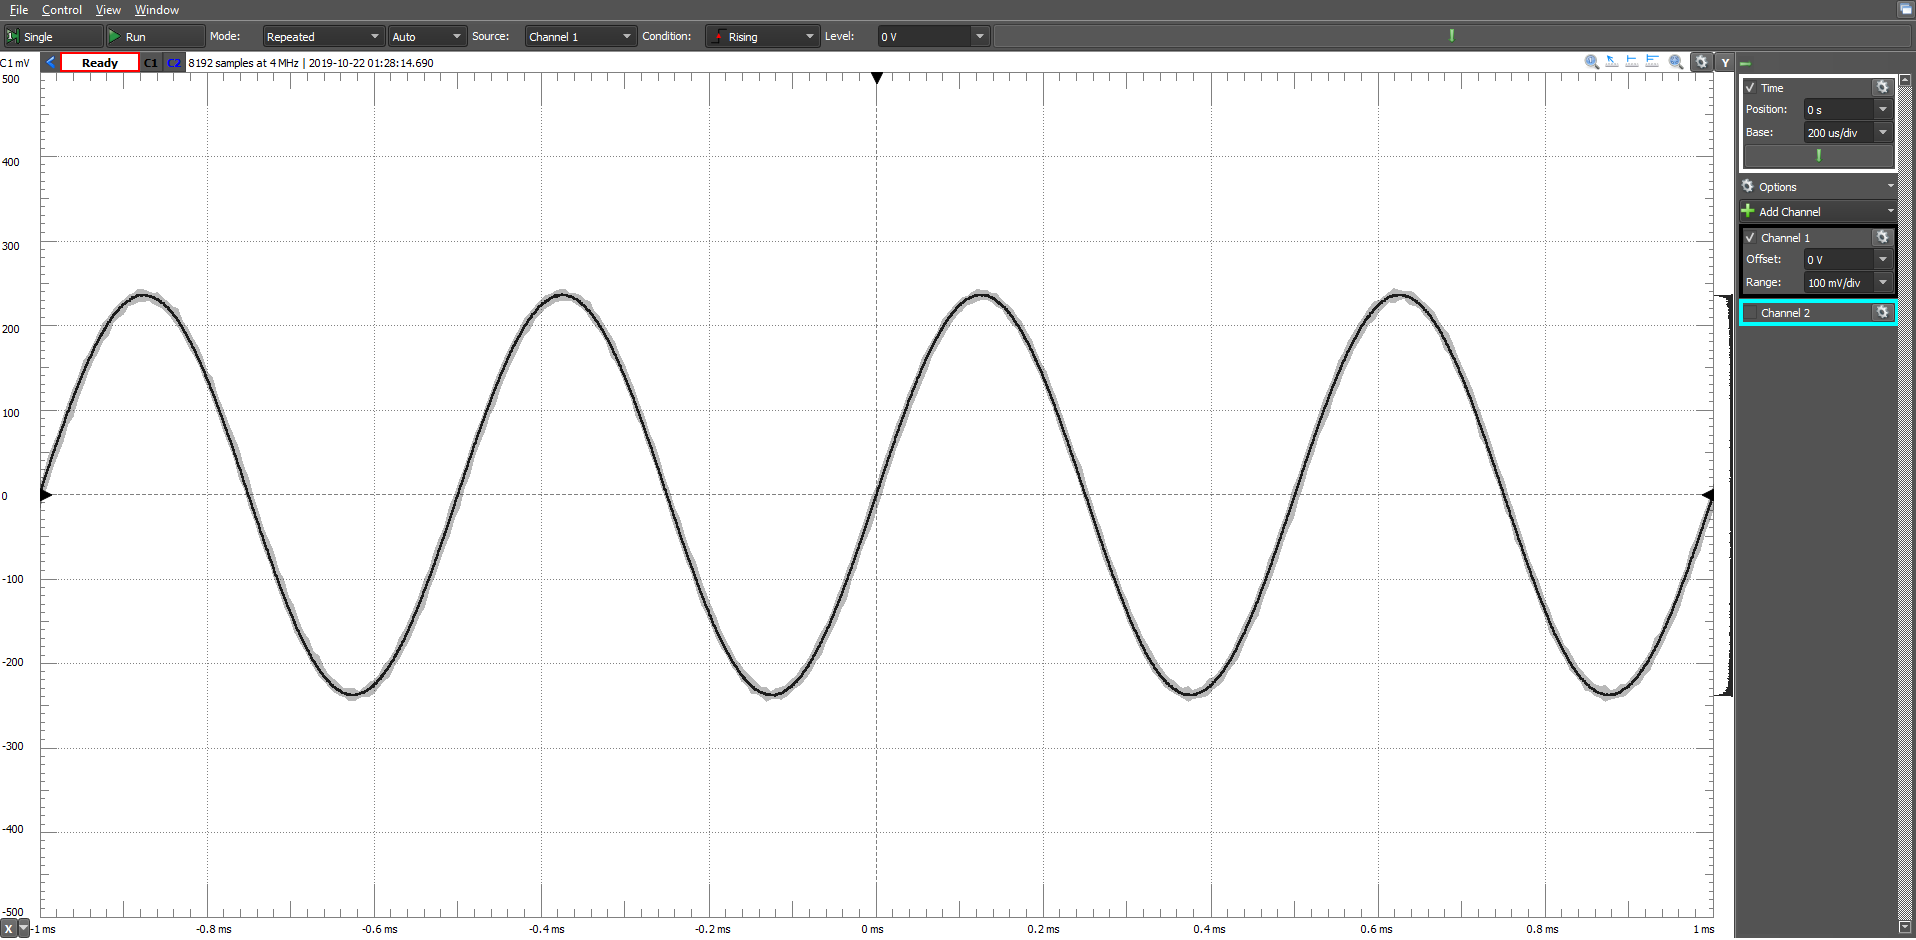
\includegraphics[width=\textwidth]{prelab5sinwave.png}

\end{document}